\documentclass[a4paper,12pt]{article}

\documentclass[a4paper,12pt]{article}

\usepackage{indentfirst}
\usepackage{cite}
\usepackage[utf8]{inputenc}
\usepackage[T1]{polski}
\usepackage{helvet}
\usepackage{graphicx}
\usepackage{svg}
\usepackage{color}
\usepackage{geometry}
\usepackage{float}
\usepackage{multirow}
\usepackage[hidelinks]{hyperref}
\usepackage{caption}
% dodaj bibliografię do spisu treści
\usepackage[nottoc]{tocbibind}
% unikaj pojedynczych linii na początku/ końcu stron
\usepackage[defaultlines=4,all]{nowidow}
\usepackage{subcaption}
\usepackage{amsmath}
\usepackage{amsfonts}

% set default figure placement to !htbp
\makeatletter
\def\fps@figure{!htbp}
\makeatother


\newcommand{\setSubtitle}[1]{
    \newcommand{\subtitle}{#1}
    }

\newcommand{\labdate}{18 listopada 2020}
\newcommand{\temat}{Stereologia}

\begin{document}
    
% Please add the following required packages to your document preamble:
% \usepackage{multirow}
% \usepackage{graphicx}

\begin{table}[]
    \resizebox{\textwidth}{!}{%
    \begin{tabular}{|c|c|c|c|}
    \hline
    \multicolumn{2}{|c|}{\multirow{2}{*}{\hspace{0.5cm} 
\includegraphics[height=2.3cm]{img/logoAGH} \hspace{0.5cm} }}                                                                    & \multicolumn{2}{c|}{\textbf{\begin{tabular}[c]{@{}c@{}} Akademia Górniczo-Hutnicza w Krakowie\\ Wydział Inżynierii Materiałowe i Ceramiki  \vspace{0.5cm} \end{tabular}}}                                     \\ \cline{3-4} 
    \multicolumn{2}{|c|}{}                                                                                       & \multicolumn{2}{c|}{\begin{tabular}[c]{@{}c@{}}Aleksandra Barcz\\ Alicja Kotwica  \vspace{0.5cm} \end{tabular}}                                                                                              \\ \hline
    \multicolumn{4}{|c|}{\textbf{Metody Badań Materiałów}}                                                                                                                                                                                                                                                     \\ \hline
    \multicolumn{4}{|c|}{\textbf{\temat}}                                                                                                                                                                                                                                                                            \\ \hline
    \begin{tabular}[c]{@{}c@{}}Rok Akademicki:\\ 2020/2021\end{tabular}         & \multicolumn{2}{c|}{\begin{tabular}[c]{@{}c@{}}Rok studiów:\\ IV\end{tabular}}                                  & \begin{tabular}[c]{@{}c@{}}Kierunek:\\ Ceramika\end{tabular}                                                       \\ \hline
    \begin{tabular}[c]{@{}c@{}}Data wykonania ćwiczenia\\ \labdate \end{tabular} & \multicolumn{2}{c|}{\begin{tabular}[c]{@{}c@{}}Data oddania sprawozdania:\\ \today \end{tabular}} & \begin{tabular}[c]{@{}c@{}}Prowadzący:\\ Dr. inż. Beata Macherzyńska\end{tabular}                                  \\ \hline
    \end{tabular}%
    }
    \end{table}


\section{Cel ćwiczenia}

Wyznaczenie udziału objętościowego, rozwinięcie powierzchni oraz wielkości ziaren.

\section{Wprowadzenie}

Stereologia to nauka o~przestrzennej budowie materiałów i~metodach ich ilościowego opisu w~oparciu o~pomiary wykonane na płaskich przekrojach materiałów. Podstawowe parametry charakteryzujące elementy mikrostrukturę tworzywa to udział objętościowy $V_V$, rozwinięcie powierzchni $S_V$ oraz wielkość ziaren $N_A$.

Wyróżnia się {\color{purple}3} metody wyznaczania udziału objętościowego faz $V_v$, które wynikają z~równania stereologicznego:

$$V_V=A_A=L_L=P_P$$

\begin{enumerate}
    \item Metoda liniową, która polega na pomiarze sumy długości  odcinków przypadających na daną fazę i~odniesieniu jej do całkowitej długości linii przyłożonej do analizowanego zgładu. Metoda pracochłonna, ale przydatna przy określaniu udziału objętościowego faz znajdujących się w~małych ilościach i~liniowo zorientowanych. 
    \item Metoda punktową, która opiera się na rachunku prawdopodobieństwa - prawdopodobieństwo trafienia punktu rzuconego losowo na powierzchnię zgładu w~daną fazę jest równa stosunkowi powierzchni zajmowanej przez tą fazę do całej powierzchni zgładu i~nie zależy od kształtu oraz rozmieszczenia badanej fazy. Wyróżnia się 2 warianty tej metody – metodę punktów losowych oraz metodę punktów rozłożonych systematycznie (metoda siatkowa).
\end{enumerate}

\newpage

Do wyznaczenia rozwinięcia powierzchniowego wyróżnia się 2 metody:

\begin{enumerate}
    \item  Metoda siecznych przypadkowych, {\color{blue} sieczną, polega na przyłożeniu do zdjęcia mikroskopowego, z sposób nieuporządkowany kalki z nakreśloną krzywą o znanej długości. Średnia liczba przecięć z układem powierzchni odniesienia do jednostki długości jest proporcjonalna do całkowitej powierzchni układu w jednostce objętości. 
    
$$S_V=\cfrac{2p}{k\cdot l} \sum ^k_{i=1}n_i$$

gdzie:

$p$ - powiększenie

$k$ - liczba pomiarów

$l$ - długość odcinka

$n_i$ - liczba przecięć z~granicą faz
    } 
    \item  Metoda siecznych skierowanych, odpowiednio do kierunków zorientowanych osi czy płaszczyzn badanego materiału, można badać zarówno tekstury izomeryczne jak również zorientowane. W~tym przypadku można wyznaczyć średnią liczbę przecięć granic ziaren na jednostkę długości siecznych przy niewielkiej liczbie zgładów, a~ze znajomości $P_L$ wyznaczymy rozwinięcie powierzchni, jakie przypada na jednostkę objętości. Najbardziej poglądową charakterystykę orientacji układu linii na płaszczyźnie, a~zarazem bardzo czułym wskaźnikiem istnienia nawet niewielkiego zorientowania linii jest tzw. "róża liczby przecięć" zaproponowana przez Sołtykowa. Przedstawia ona zależność między średnią liczbą przecięć na jednostkową długość siecznych a~kierunkiem siecznych we współrzędnych biegunowych.
\end{enumerate}

W~celu wyznaczenia wielkości ziaren  stosujemy:

\begin{enumerate}
    \item Metoda odwrotności średnic Sołtykowa, która polega na zmierzeniu średnicy wszystkich przekrojów badanych ziaren znajdujących się na powierzchni zgładu. Pomiary średnicy dla każdego ziarna wykonać należy  w~dwu wzajemnie prostopadłych kierunkach.
    \newpage
    \item Metoda Jeffriesa, która jest najprostsza. Na obraz zgładu nanosimy prostokąt o~bokach a~i~b,~który dzieli nam ziarna na trzy grupy: z,~w~i~u.{\color{blue} 
    
    $$N_A=\cfrac{p^2}{a\cdot b}(z+0.5w+0.25u)$$
    
    gdzie: 
    
    p-powiększenie
    
    z-liczba ziaren leżących całkowicie wewnątrz prostokąta
    
    w-liczba ziaren przeciętych przez brzegi prostokąta 
    
    u-liczba ziaren leżących w~narożach prostokąta
    
    $a$ i~$b$ - długość boków prostokąta,
    
    } 
    
   {\color{blue} Do określania $N_V$ stosujemy metodę odwrotności średnic Sałtykowa. Do jej użycia konieczne jest wyznaczenie wszystkich średnic mierzonych ziaren. Mierzy się je ziarna wzdłuż i wszerz i dzieli się sumę tych wyników przez 2. Ze zmierzonych średnic, gdy mamy znaczną ich liczbę, buduje się szereg rozdzielczy o średnicach przekrojów $d_i$ i liczebności $N_i$. Liczbę wylicza się ze wzoru danego przez Sałtykowa: 
   $$N_V=\cfrac{2}{\pi}\cdot \overline{d^{-1}} \cdot N_A$$
   
   $N_V$ - liczba ziaren na jednostkę objętości
   }
   \newline
   
   
\end{enumerate}


Literatura

Metody Badań "Mikroskopia Optyczna" część B,~Jan Piekarczyk

\newpage

\section{Aparatura i~materiały}

Aparatura:
\begin{itemize}
    \item komputer
\end{itemize}

Materiały:
\begin{itemize}
    \item linijka,
    \item kątomierz,
    \item kalka techniczna,
    \item mikrostruktura kompozytu włókno C/żywica epoksydowa
    \item mikrostruktura grafitu $p=300x$
\end{itemize}


\section{Wyniki i~obliczenia}

\subsection{Udział objętościowy $V_V$}

Na kalce narysowałyśmy siatkę o~oczkach $1.5$ x~$1.5 cm$. Następnie przyłożyłyśmy siatkę do wydrukowanej kartki i~zaznaczyłyśmy przecięcia z~faza włókna C/żywica epoksydowa, na tej podstawie wyznaczyłyśmy udziały objętościowe faz i~minimalną ilość przyłożeń siatki. Pomiary powtórzyłyśmy jeszcze 9 razy używając różnych wartości węzłów. Podobne czynności przeprowadzono dla metody liniowej. Odcinek o~długości $10cm$ przykładałyśmy w~przypadkowych miejscach, a~następnie zliczyłyśmy punkty przecięcia. 

Na podstawie otrzymanych wyników obliczyłyśmy udział objętościowy fazy $\alpha$, a~następnie obliczyłyśmy szacunkową minimalną wartość przyłożeń siatki ze wzoru:

$$n\ge \cfrac{t^2 \cdot (1-V_V(\alpha))}{\gamma^2 \cdot k~\cdot V_V(\alpha)}$$

gdzie:

$n$ - szacunkowa minimalna liczba przyłożeń siatki

$k$ - liczba węzłów siatki

$V_V(\alpha)$ - udział objętościowy fazy $\alpha$

$\gamma$ - błąd względny wynoszący $0.05$, dla prawdopodobieństwa $95\%$ $(t=1.96)$
\newpage

$$\mu=\overline{V}\pm t~\cdot s(\overline{V})=\overline{V}\pm \cfrac{t\cdot s}{\sqrt{n}}=\overline{V}\pm \delta = \overline{V}\pm \gamma \cdot \overline{V}$$

Gdzie:

$\gamma=\cfrac{t\cdot s}{\overline{V}\cdot \sqrt{n}}$

$\overline{V}$ - wyliczona średnia dla próbki pobranej populacji

$s(\overline{V})$ - oszacowany błąd standardowy

$s$ - oszacowane odchylenie standardowe

$x$ - wartości mierzone 

$n$ - liczba pomiarów

$t$ - zmienna standaryzowana ($t=1.96$ dla prawdopodobieństwa $95\%$ $\alpha=0.05$)

$\delta$ - błąd bezwzględny

$\gamma$ - błąd względny

$s=\sqrt{\cfrac{\Sigma (V-\overline{V})^2}{n-1}}$

\begin{figure}[H]
    \centering
    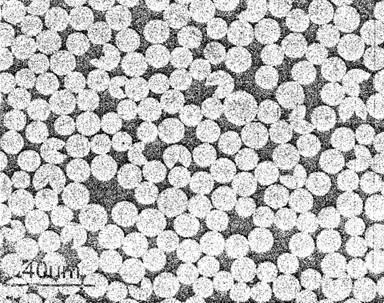
\includegraphics[width=0.7\textwidth]{img/VV.png}
\end{figure}

\newpage

\subsubsection{Metoda punktowa}

{\color{purple}
Stworzona siatka zawsze była obejmowana cała przez zdjęcie, a więc liczba punktów leżących na zdjęciu zawsze wynosiła $k=42$. }

{\color{blue} Za pomocą wzoru podanego poniżej policzyliśmy szacunkową minimalną wartość przyłożeń siatki.
$$n\ge \cfrac{t^2 \cdot (1-V_V(\alpha))}{\gamma^2 \cdot k~\cdot V_V(\alpha)}$$

$$n\ge \cfrac{1.96^2 \cdot (1-0.16)}{0.05^2 \cdot 42~\cdot 0.16}$$
}

Po dokonanych obliczeniach wiemy, że szacunkowa minimalna wartość przyłożeń siatki wynosi $n\ge 193$.

% Please add the following required packages to your document preamble:
% \usepackage{graphicx}
\begin{table}[H]
\centering
\caption{Udział objętościowy fazy $\alpha$ dla metody punktowej.}
\label{tab:my-table}
\resizebox{0.7\textwidth}{!}{%
\begin{tabular}{|r|r|r|r|r}
\hline
\multicolumn{1}{|c|}{L.P} & \multicolumn{1}{c|}{$z(\alpha)$} & \multicolumn{1}{c|}{$k$} & \multicolumn{1}{c|}{$V_V(\alpha)$} & \multicolumn{1}{c|}{$(V-\overline{V}$)} \\ \hline
1                         & 6                                & 42                       & 0,14                               & \multicolumn{1}{r|}{-0,02}                               \\ \hline
2                         & 8                                & 42                       & 0,19                               & \multicolumn{1}{r|}{0,03}                                \\ \hline
3                         & 6                                & 42                       & 0,14                               & \multicolumn{1}{r|}{-0,02}                               \\ \hline
4                         & 7                                & 42                       & 0,17                               & \multicolumn{1}{r|}{0,01}                                \\ \hline
5                         & 7                                & 42                       & 0,17                               & \multicolumn{1}{r|}{0,01}                                \\ \hline
6                         & 8                                & 42                       & 0,19                               & \multicolumn{1}{r|}{0,03}                                \\ \hline
7                         & 5                                & 42                       & 0,12                               & \multicolumn{1}{r|}{-0,04}                               \\ \hline
8                         & 5                                & 42                       & 0,12                               & \multicolumn{1}{r|}{-0,04}                               \\ \hline
9                         & 7                                & 42                       & 0,17                               & \multicolumn{1}{r|}{0,01}                                \\ \hline
10                        & 8                                & 42                       & 0,19                               & \multicolumn{1}{r|}{0,03}                                \\ \hline
\multicolumn{3}{|c|}{Wartość średnia $\overline{V}$}                   & 0,16                               & \multicolumn{1}{l}{}                                     \\ \cline{1-4}
\multicolumn{3}{|c|}{Odchylenie standardowe $s$}                                        & 0,03                               & \multicolumn{1}{l}{}                                     \\ \cline{1-4}
\end{tabular}%
}
\end{table}

Przedział ufności dla metody punktowej wynosi $\mu=0.16\pm 0.0541$.

Błąd względny wynosi $\gamma=0.1073$.
\newpage

\subsubsection{Metoda liniowa}

{\color{blue} Za pomocą wzoru podanego poniżej policzyliśmy szacunkową minimalną wartość przyłożeń linii.
$$n\ge \cfrac{t^2 \cdot (1-V_V(\alpha))}{\gamma^2 \cdot k~\cdot V_V(\alpha)}$$

$$n\ge \cfrac{1.96^2 \cdot (1-0.23)}{0.05^2 \cdot 100~\cdot 0.23}$$
}

Po dokonanych obliczeniach wiemy, że szacunkowa minimalna wartość przyłożeń linii wynosi $n\ge 51$.

% Please add the following required packages to your document preamble:
% \usepackage{graphicx}
\begin{table}[H]
\centering
\caption{Udział objętościowy fazy $\alpha$ dla metody liniowej}
\label{tab:my-table}
\resizebox{0.7\textwidth}{!}{%
\begin{tabular}{|r|r|r|r|r}
\hline
\multicolumn{1}{|l|}{L.P} & \multicolumn{1}{l|}{$z(\alpha)$ {[}mm{]}} & \multicolumn{1}{l|}{$k$ {[}mm{]}} & \multicolumn{1}{l|}{$V_V(\alpha)$} & \multicolumn{1}{l|}{$(V-\overline{V})$} \\ \hline
1                         & 15                                        & 100                               & 0,15                               & \multicolumn{1}{r|}{-0,08}                               \\ \hline
2                         & 25                                        & 100                               & 0,25                               & \multicolumn{1}{r|}{0,02}                                \\ \hline
3                         & 27                                        & 100                               & 0,27                               & \multicolumn{1}{r|}{0,04}                                \\ \hline
4                         & 29                                        & 100                               & 0,29                               & \multicolumn{1}{r|}{0,06}                                \\ \hline
5                         & 24                                        & 100                               & 0,24                               & \multicolumn{1}{r|}{0,01}                                \\ \hline
6                         & 12                                        & 100                               & 0,12                               & \multicolumn{1}{r|}{-0,11}                               \\ \hline
7                         & 28                                        & 100                               & 0,28                               & \multicolumn{1}{r|}{0,05}                                \\ \hline
8                         & 27                                        & 100                               & 0,27                               & \multicolumn{1}{r|}{0,04}                                \\ \hline
9                         & 28                                        & 100                               & 0,28                               & \multicolumn{1}{r|}{0,05}                                \\ \hline
10                        & 17                                        & 100                               & 0,17                               & \multicolumn{1}{r|}{-0,06}                               \\ \hline
\multicolumn{3}{|l|}{Wartość średnia $\overline{V}$}                                     & 0,23                               & \multicolumn{1}{l}{}                                     \\ \cline{1-4}
\multicolumn{3}{|l|}{Odchylenie standardowe $S$}                                                          & 0,06                               & \multicolumn{1}{l}{}                                     \\ \cline{1-4}
\end{tabular}%
}
\end{table}

Przedział ufności dla metody punktowej wynosi $\mu=0.23\pm 0.1211$.

Błąd względny wynosi $\gamma=0.1651$.
\newpage

{\color{purple}
\subsubsection{Podsumowanie i wnioski}

% Please add the following required packages to your document preamble:
% \usepackage{graphicx}
\begin{table}[H]
\centering
\caption{Porównanie wyników udziału objętościowego $V_V$.}
\label{tab:my-table}
\resizebox{0.7\textwidth}{!}{%
\begin{tabular}{|c|r|r|r|r|}
\hline
Metoda   & \multicolumn{1}{c|}{$V_V(\alpha)$} & \multicolumn{1}{c|}{$\mu$} & \multicolumn{1}{c|}{$n$} & \multicolumn{1}{c|}{$\gamma$} \\ \hline
Punktowa & 0.16                                               & 0.16$\pm$0.0541            & 193                      & 0.1073                        \\ \hline
Liniowa  & 0.23                                               & 0.23$\pm$0.1211            & 51                       & 0.1651                        \\ \hline
\end{tabular}%
}
\end{table}

Obydwie metody, zarówno metoda liniowa jak i~punktowa, dały podobne  do siebie wyniki wartości udziału fazy $\alpha$ (różnią się wartością około $0.07$), co może świadczyć, że metody są do siebie zbliżone. W~przypadku metody punktowej błąd względny wynosi  około $0.10$, nie jest to duży błąd, świadczy to  o~dokładności przeprowadzonych obliczeń, natomiast w~metodzie liniowej błąd względny wynosi  $0.16$, jest on wyższy niż w~metodzie punktowej. Przyczyną mogła być niedokładność  podczas wykonywania  ćwiczenia spowodowana niepoprawnym odczytaniem wyników lub złego przyłożenia linijki.}
\newpage

\subsection{Rozwinięcie powierzchni $S_V$}

Na kartce narysowaliśmy linię $10cm$, a~następnie przyłożyłyśmy do zdjęcia i~policzyłyśmy ilość przeciętych granic międzyziarnowych. Później wykonałyśmy poniższe obliczenia, a~wyniki zestawiłyśmy w~tabeli 4.  Natomiast w~metodzie siecznych skierowanych na kartce narysowaliśmy linie o~długości $5cm$. Następnie za pomocą kątomierza narysowano 5 linii, każda o~długości $5cm$, pod kątami $30^\circ$, $60^\circ$, $90^\circ$, $120^\circ$ i~$150^\circ$. Przyłożono do fotografii i~zmierzono 10-krotnie liczbę przecięć z~każdą linia. Wyniki zanotowano w~tabeli 2.
Powiększenie zdjęcia  wynosi 300x , które zastosowano w~obliczeniach.
\newline

Przedział ufności dla obydwóch pomiarów został policzony ze wzoru:
$$\mu = S_V\pm t\cdot s$$
\newline 

Błąd względny dla obydwóch pomiarów policzono ze wzoru:

$$\gamma=\cfrac{t\cdot s}{S_V\cdot \sqrt{n}}$$

\begin{figure}[H]
    \centering
    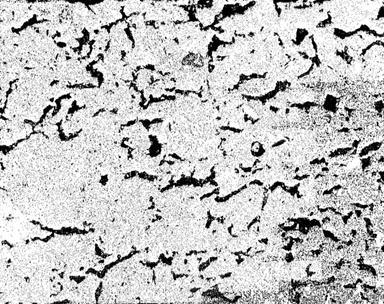
\includegraphics[width=0.7\textwidth]{img/SV.png}
\end{figure}


\subsubsection{Pomiar rozwinięcia powierzchni}

W~celu obliczenia ilości przecięć na jednostkę długości odcinka wykorzystaliśmy wzór:

$$P_L=\cfrac{P}{L}$$

Gdzie:

$P$ - ilość przeciętych granic międzyziarnowych

$L$ - długość odcinka w~cm.

Do policzenia rozwinięcia powierzchni wykorzystaliśmy wzór:

$$S_V=\cfrac{2p}{k\cdot l} \sum ^k_{i=1}n_i$$

gdzie:

{\color{purple}$p$ - powiększenie ($p=300x$)}

$k$ - liczba pomiarów

$l$ - długość odcinka

$n_i$ - liczba przecięć z~granicą faz

% Please add the following required packages to your document preamble:
% \usepackage{graphicx}
\begin{table}[H]
\centering
\caption{Rozwinięcie powierzchni.}
\label{tab:my-table}
\resizebox{0.7\textwidth}{!}{%
\begin{tabular}{|c|l|r|r|r|}
\hline
L.P & \multicolumn{1}{c|}{$P$} & \multicolumn{1}{c|}{$L$ {[}cm{]}} & \multicolumn{1}{c|}{$P_L$ $[cm^{-1}]$} & \multicolumn{1}{c|}{$S_V$ $[cm^2/cm^3]$} \\ \hline
1   & 17                       & 10                                & 1,7                                    & 1020                                   \\ \hline
2   & 17                       & 10                                & 1,7                                    & 1020                                   \\ \hline
3   & 26                       & 10                                & 2,6                                    & 1560                                   \\ \hline
4   & 22                       & 10                                & 2,2                                    & 1320                                   \\ \hline
5   & 12                       & 10                                & 1,2                                    & 720                                    \\ \hline
6   & 16                       & 10                                & 1,6                                    & 960                                    \\ \hline
7   & 9                        & 10                                & 0,9                                    & 540                                    \\ \hline
8   & 10                       & 10                                & 1,0                                    & 600                                    \\ \hline
9   & 22                       & 10                                & 2,2                                    & 1320                                   \\ \hline
10  & 22                       & 10                                & 2,2                                    & 1320                                   \\ \hline
\multicolumn{4}{|c|}{Wartość średnia $\overline{S}_V$}                                                      & 1038,0                                   \\ \hline
\multicolumn{4}{|c|}{Odchylenie standardowe $s$}                                                            & 343,0                                    \\ \hline
\multicolumn{4}{|c|}{Przedział ufności $\mu$}                                                               & 1038,0$\pm$672,25                      \\ \hline
\end{tabular}%
}
\end{table}
\newpage

Błąd względny wyniósł:

$$\gamma=0.20$$

\subsubsection{Pomiar orientacji powierzchni granicznych}

W~celu obliczenia ilości przecięć na jednostkę długości odcinka wykorzystaliśmy wzór:

$$P_L=\cfrac{P}{L} \cdot p$$

Gdzie:

$P$ - ilość przeciętych granic międzyziarnowych,

$L$ - długość odcinka w~cm,

$p$ - powiększenie.
\newline

Do policzenia rozwinięcia powierzchni wykorzystaliśmy wzór:

$$S_V= 2\cdot P_L$$

% Please add the following required packages to your document preamble:
% \usepackage{graphicx}
% \usepackage[table.xcdraw]{xcolor}
% If you use beamer only pass "xcolor=table" option. i.e. \documentclass[xcolor=table]{beamer}
\begin{table}[H]
    \centering
    \caption{Pomiar orientacji powierzchni.}
    \label{tab:my-table}
    \resizebox{0.7\textwidth}{!}{%
    \begin{tabular}{|c|r|r|r|r|r|r|l}
    \cline{1-7}
    Kąt   & \multicolumn{1}{c|}{$0^\circ$} & \multicolumn{1}{c|}{$30^\circ$} & \multicolumn{1}{c|}{$60^\circ$} & \multicolumn{1}{c|}{$90^\circ$} & \multicolumn{1}{c|}{$120^\circ$} & \multicolumn{1}{c|}{$150^\circ$} &                  \\ \cline{1-7}
    1     & 9                              & 5                                                    & 9                                                    & 7                                                    & 15                                                    & 7                                                     &                                       \\ \cline{1-7}
    2     & 5                              & 8                                                    & 8                                                    & 6                                                    & 8                                                     & 2                                                     &                                       \\ \cline{1-7}
    3     & 6                              & 4                                                    & 9                                                    & 6                                                    & 12                                                    & 5                                                     &                                       \\ \cline{1-7}
    4     & 9                              & 11                                                   & 11                                                   & 7                                                    & 9                                                     & 8                                                     &                                       \\ \cline{1-7}
    5     & 9                              & 4                                                    & 8                                                    & 6                                                    & 7                                                     & 5                                                     &                                       \\ \cline{1-7}
    6     & 9                              & 9                                                    & 6                                                    & 6                                                    & 7                                                     & 1                                                     &                                       \\ \cline{1-7}
    7     & 6                              & 8                                                    & 13                                                   & 7                                                    & 9                                                     & 4                                                     &                                       \\ \cline{1-7}
    8     & 5                              & 5                                                    & 13                                                   & 6                                                    & 7                                                     & 1                                                     &                                       \\ \cline{1-7}
    9     & 9                              & 12                                                   & 5                                                    & 6                                                    & 7                                                     & 9                                                     &                                       \\ \cline{1-7}
    10    & 12                             & 6                                                    & 8                                                    & 6                                                    & 8                                                     & 3                                                     & \multicolumn{1}{r}{}                  \\ \hline
    Średnia  & 7.9                             & 7.2                                                   & 9.0                                                   & 6.3                                                   & 8.9                                                    & 4.5                                                    & \multicolumn{1}{c|}{$\overline{P}_L$ i $\overline{S}_V$} \\ \hline
    $P_L$ & 474                           & 432                                                 & 540                                                  & 378                                                 & 534                                                  & 270                                                   & \multicolumn{1}{r|}{438}             \\ \hline
    $S_V$ & 948                           & 864                                                 & 1080                                                  & 756                                                 & 1068                                                  & 540                                                   & \multicolumn{1}{r|}{876}             \\ \hline
    \end{tabular}%
    }
    \end{table}

Odchylenie standardowe dla pomiaru orientacji powierzchni granicznych 

wynosi:
$$s=205.48$$

Przedział ufności dla pomiaru orientacji powierzchni granicznych wynosi:
$$\mu = 876\pm 402.73$$

Błąd względny dla pomiaru orientacji powierzchni granicznych wynosi:
$$\gamma = 0.15$$
\newline

\begin{figure}[H]
    \centering
    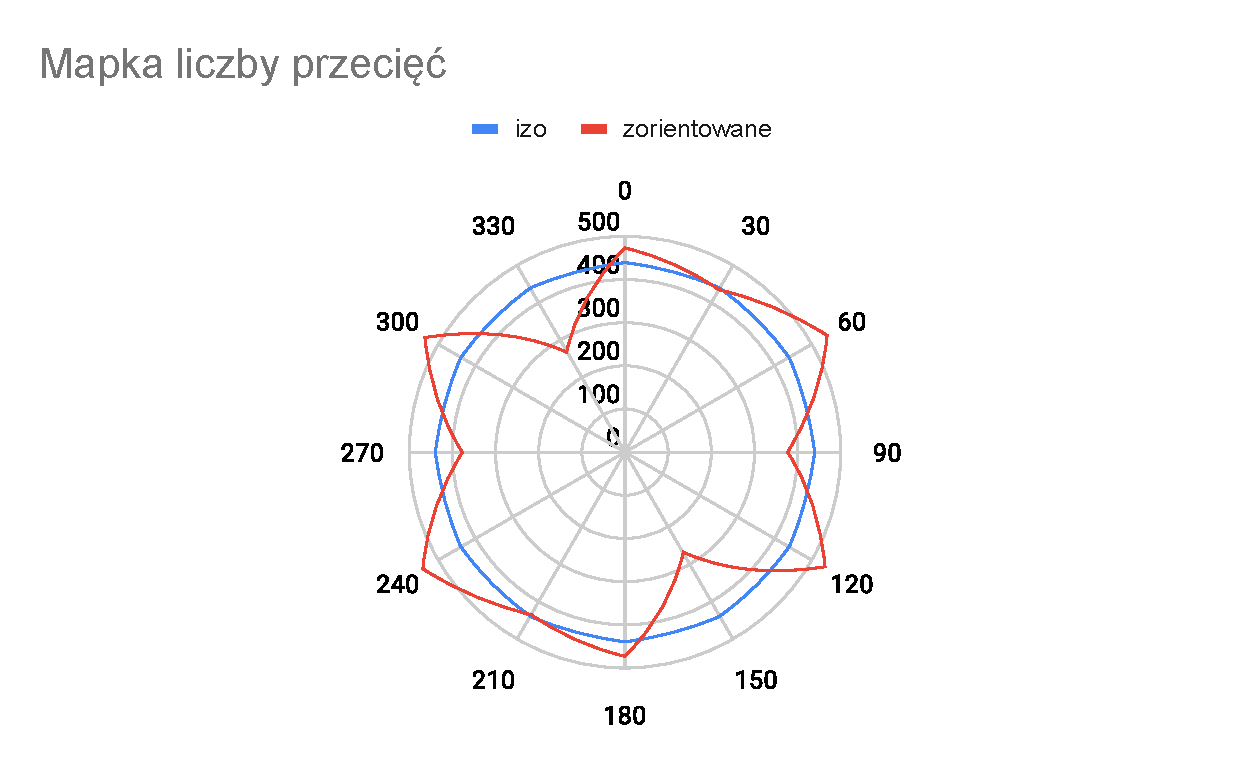
\includegraphics[width=\textwidth]{img/Mapka liczby przecięć.pdf}
\end{figure}

{\color{purple}
Na podstawie mapki przecięć widzimy, że najmniej przecięć jest przy $150^{\circ}$. Nie jesteśmy w stanie stwierdzić na podstawie tego wykresu w jakim kierunku jest ziarno spłaszczone. Widzimy również, że ziarna nie są ukierunkowane w~jedną stronę, tylko w~trzy. 
}

\newpage
{\color{purple}
\subsubsection{Podsumowanie i wnioski}

% Please add the following required packages to your document preamble:
% \usepackage{graphicx}
\begin{table}[H]
\centering
\caption{Porównanie wyników rozwinięcia powierzchni $S_V$.}
\label{tab:my-table}
\resizebox{\textwidth}{!}{%
\begin{tabular}{|c|r|r|r|r|}
\hline
Metoda                  & \multicolumn{1}{c|}{$\overline{S}_V$} & \multicolumn{1}{c|}{$s$} & \multicolumn{1}{c|}{$\mu$} & \multicolumn{1}{c|}{$\gamma$} \\ \hline
Siecznych przypadkowych & 1038 .0                                & 343.0                    & $1038.0\pm 672.25$           & 0.20                          \\ \hline
Siecznych skierowanych  & 876                                   & 205.48                   & $876\pm 402.73$            & 0.15                          \\ \hline
\end{tabular}%
}
\end{table}

Dzięki znajomości ilości przecięć na dany odcinek oraz uwzględniając powiększenie otrzymanej mikrofotografii, mogłyśmy obliczyć rozwinięcie powierzchni materiału porowatego. Niektóre z~obliczonych wartości znacznie się od siebie różnią, te rozbieżności spowodowały tak duże wartości przedziału ufności i~odchylenia standardowego.{\color{blue} W~metodzie siecznych przypadkowych rozwiniecie powierzchni jest większe niż w~przypadku metodzie siecznych skierowanych, różnica wynosi 162.}}
\newpage

\subsection{Wielkość ziaren}

Zmierzono średnicę wszystkich nie przeciętych brzegiem zdjęcia ziaren. Wykonano pomiar w~dwóch prostopadłych kierunkach, a~następnie wyliczono wartość średnią $d$ dla każdego ziarna. Wyniki zestawiono w~tabeli 5.

Znaleźliśmy ziarno z~największą średnicą $d_{max}$, którym jest ziarno numer 93 i~podzieliliśmy tą wielkość na osiem równych części, dzięki czemu ustaliliśmy wartości przedziałów. Pogrupowano wyniki do odpowiednich przedziałów i~wyliczono średnicę przekrojów $d_i$, która jest środkową wartością każdego przedziału i~jej odwrotność. Wykonano pozostałe obliczenia uwzględniając powiększenie p=1200. Wyniki zestawiono w~tabeli 8.
Następnie wyliczono parametry przestrzenne ziaren: liczbę ziaren na jednostkę objętości $N_V$, średnią wielkość ziaren $\overline{D}$, średnie odchylenie kwadratowe średnic ziaren $\sigma D$ oraz udział objętościowy $V_V$.

Następnie wyliczono parametry przestrzenne ziaren: liczbę ziaren na jednostkę objętości $N_V$, średnią wielkość ziaren $\overline{D}$, średnie odchylenie kwadratowe oraz udział objętościowy $V_V$.

Wartość $d$ policzyliśmy ze wzoru:

$$d=\cfrac{l+m}{2}$$

gdzie:

$l$ i~$k$ - wymiary prostopadłych do siebie średnic ziarna

\begin{figure}[H]
    \centering
    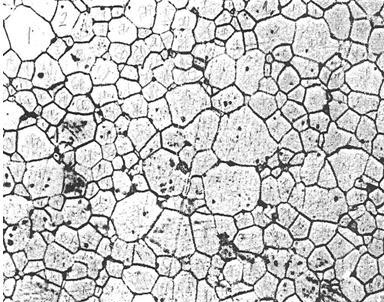
\includegraphics[width=0.7\textwidth]{img/wielkosc.png}
\end{figure}

% Please add the following required packages to your document preamble:
% \usepackage{graphicx}
\begin{table}[H]
\centering
\caption{Zestawienie wymiarów ziaren.}
\label{tab:my-table}
\resizebox{\textwidth}{!}{%
\begin{tabular}{|c|r|r|r|l|c|r|r|r|l|c|r|r|r|lcrrr}
\cline{1-4} \cline{6-9} \cline{11-14} \cline{16-19}
\begin{tabular}[c]{@{}c@{}}nr. \\ ziarna\end{tabular} & \multicolumn{1}{c|}{\begin{tabular}[c]{@{}c@{}}$l$\\ $[mm]$\end{tabular}} & \multicolumn{1}{c|}{\begin{tabular}[c]{@{}c@{}}$m$\\ $[mm]$\end{tabular}} & \multicolumn{1}{c|}{\begin{tabular}[c]{@{}c@{}}$d$\\ $[mm]$\end{tabular}} &  & 55  & 7,0  & 6,0  & 6,5  &  & 110 & 6,0  & 6,0  & 6,0  & \multicolumn{1}{l|}{} & \multicolumn{1}{c|}{165} & \multicolumn{1}{r|}{6,0}  & \multicolumn{1}{r|}{5,0}  & \multicolumn{1}{r|}{5,5}  \\ \cline{1-4} \cline{6-9} \cline{11-14} \cline{16-19} 
1                                                     & 12,0                                                                      & 13,0                                                                      & 12,5                                                                      &  & 56  & 5,0  & 4,0  & 4,5  &  & 111 & 4,0  & 8,0  & 6,0  & \multicolumn{1}{l|}{} & \multicolumn{1}{c|}{166} & \multicolumn{1}{r|}{7,0}  & \multicolumn{1}{r|}{6,0}  & \multicolumn{1}{r|}{6,5}  \\ \cline{1-4} \cline{6-9} \cline{11-14} \cline{16-19} 
2                                                     & 6,0                                                                       & 4,0                                                                       & 5,0                                                                       &  & 57  & 5,0  & 3,0  & 4,0  &  & 112 & 6,0  & 5,0  & 5,5  & \multicolumn{1}{l|}{} & \multicolumn{1}{c|}{167} & \multicolumn{1}{r|}{10,0} & \multicolumn{1}{r|}{13,0} & \multicolumn{1}{r|}{11,5} \\ \cline{1-4} \cline{6-9} \cline{11-14} \cline{16-19} 
3                                                     & 5,0                                                                       & 3,0                                                                       & 4,0                                                                       &  & 58  & 8,0  & 7,0  & 7,5  &  & 113 & 6,0  & 5,0  & 5,5  & \multicolumn{1}{l|}{} & \multicolumn{1}{c|}{168} & \multicolumn{1}{r|}{10,0} & \multicolumn{1}{r|}{6,0}  & \multicolumn{1}{r|}{8,0}  \\ \cline{1-4} \cline{6-9} \cline{11-14} \cline{16-19} 
4                                                     & 1,0                                                                       & 1,0                                                                       & 1,0                                                                       &  & 59  & 5,0  & 4,0  & 4,5  &  & 114 & 7,0  & 6,0  & 6,5  & \multicolumn{1}{l|}{} & \multicolumn{1}{c|}{169} & \multicolumn{1}{r|}{4,0}  & \multicolumn{1}{r|}{5,0}  & \multicolumn{1}{r|}{4,5}  \\ \cline{1-4} \cline{6-9} \cline{11-14} \cline{16-19} 
5                                                     & 5,0                                                                       & 7,0                                                                       & 6,0                                                                       &  & 60  & 6,0  & 7,0  & 6,5  &  & 115 & 6,0  & 6,0  & 6,0  & \multicolumn{1}{l|}{} & \multicolumn{1}{c|}{170} & \multicolumn{1}{r|}{5,0}  & \multicolumn{1}{r|}{6,0}  & \multicolumn{1}{r|}{5,5}  \\ \cline{1-4} \cline{6-9} \cline{11-14} \cline{16-19} 
6                                                     & 3,0                                                                       & 5,0                                                                       & 4,0                                                                       &  & 61  & 7,0  & 5,0  & 6,0  &  & 116 & 10,0 & 5,0  & 7,5  & \multicolumn{1}{l|}{} & \multicolumn{1}{c|}{171} & \multicolumn{1}{r|}{5,0}  & \multicolumn{1}{r|}{7,0}  & \multicolumn{1}{r|}{6,0}  \\ \cline{1-4} \cline{6-9} \cline{11-14} \cline{16-19} 
7                                                     & 2,0                                                                       & 1,0                                                                       & 1,5                                                                       &  & 62  & 7,0  & 5,0  & 6,0  &  & 117 & 5,0  & 5,0  & 5,0  & \multicolumn{1}{l|}{} & \multicolumn{1}{c|}{172} & \multicolumn{1}{r|}{2,0}  & \multicolumn{1}{r|}{2,0}  & \multicolumn{1}{r|}{2,0}  \\ \cline{1-4} \cline{6-9} \cline{11-14} \cline{16-19} 
8                                                     & 9,0                                                                       & 9,0                                                                       & 9,0                                                                       &  & 63  & 5,0  & 5,0  & 5,0  &  & 118 & 5,0  & 6,0  & 5,5  & \multicolumn{1}{l|}{} & \multicolumn{1}{c|}{173} & \multicolumn{1}{r|}{6,0}  & \multicolumn{1}{r|}{2,0}  & \multicolumn{1}{r|}{4,0}  \\ \cline{1-4} \cline{6-9} \cline{11-14} \cline{16-19} 
9                                                     & 3,0                                                                       & 2,0                                                                       & 2,5                                                                       &  & 64  & 4,0  & 5,0  & 4,5  &  & 119 & 9,0  & 6,0  & 7,5  & \multicolumn{1}{l|}{} & \multicolumn{1}{c|}{174} & \multicolumn{1}{r|}{5,0}  & \multicolumn{1}{r|}{8,0}  & \multicolumn{1}{r|}{6,5}  \\ \cline{1-4} \cline{6-9} \cline{11-14} \cline{16-19} 
10                                                    & 5,0                                                                       & 4,0                                                                       & 4,5                                                                       &  & 65  & 4,0  & 4,0  & 4,0  &  & 120 & 9,0  & 6,0  & 7,5  & \multicolumn{1}{l|}{} & \multicolumn{1}{c|}{175} & \multicolumn{1}{r|}{4,0}  & \multicolumn{1}{r|}{5,0}  & \multicolumn{1}{r|}{4,5}  \\ \cline{1-4} \cline{6-9} \cline{11-14} \cline{16-19} 
11                                                    & 4,0                                                                       & 2,0                                                                       & 3,0                                                                       &  & 66  & 4,0  & 4,0  & 4,0  &  & 121 & 8,0  & 8,0  & 8,0  & \multicolumn{1}{l|}{} & \multicolumn{1}{c|}{176} & \multicolumn{1}{r|}{10,0} & \multicolumn{1}{r|}{8,0}  & \multicolumn{1}{r|}{9,0}  \\ \cline{1-4} \cline{6-9} \cline{11-14} \cline{16-19} 
12                                                    & 12,0                                                                      & 10,0                                                                      & 11,0                                                                      &  & 67  & 4,0  & 5,0  & 4,5  &  & 122 & 9,0  & 4,0  & 6,5  & \multicolumn{1}{l|}{} & \multicolumn{1}{c|}{177} & \multicolumn{1}{r|}{6,0}  & \multicolumn{1}{r|}{9,0}  & \multicolumn{1}{r|}{7,5}  \\ \cline{1-4} \cline{6-9} \cline{11-14} \cline{16-19} 
13                                                    & 4,0                                                                       & 2,0                                                                       & 3,0                                                                       &  & 68  & 5,0  & 8,0  & 6,5  &  & 123 & 5,0  & 6,0  & 5,5  & \multicolumn{1}{l|}{} & \multicolumn{1}{c|}{178} & \multicolumn{1}{r|}{8,0}  & \multicolumn{1}{r|}{3,0}  & \multicolumn{1}{r|}{5,5}  \\ \cline{1-4} \cline{6-9} \cline{11-14} \cline{16-19} 
14                                                    & 5,0                                                                       & 6,0                                                                       & 5,5                                                                       &  & 69  & 3,0  & 3,0  & 3,0  &  & 124 & 3,0  & 2,0  & 2,5  & \multicolumn{1}{l|}{} & \multicolumn{1}{c|}{179} & \multicolumn{1}{r|}{2,0}  & \multicolumn{1}{r|}{2,0}  & \multicolumn{1}{r|}{2,0}  \\ \cline{1-4} \cline{6-9} \cline{11-14} \cline{16-19} 
15                                                    & 7,0                                                                       & 7,0                                                                       & 7,0                                                                       &  & 70  & 3,0  & 2,0  & 2,5  &  & 125 & 3,0  & 2,0  & 2,5  & \multicolumn{1}{l|}{} & \multicolumn{1}{c|}{180} & \multicolumn{1}{r|}{7,0}  & \multicolumn{1}{r|}{2,0}  & \multicolumn{1}{r|}{4,5}  \\ \cline{1-4} \cline{6-9} \cline{11-14} \cline{16-19} 
16                                                    & 3,0                                                                       & 2,0                                                                       & 2,5                                                                       &  & 71  & 3,0  & 5,0  & 4,0  &  & 126 & 15,0 & 14,0 & 14,5 & \multicolumn{1}{l|}{} & \multicolumn{1}{c|}{181} & \multicolumn{1}{r|}{7,0}  & \multicolumn{1}{r|}{5,0}  & \multicolumn{1}{r|}{6,0}  \\ \cline{1-4} \cline{6-9} \cline{11-14} \cline{16-19} 
17                                                    & 6,0                                                                       & 3,0                                                                       & 4,5                                                                       &  & 72  & 4,0  & 3,0  & 3,5  &  & 127 & 8,0  & 6,0  & 7,0  & \multicolumn{1}{l|}{} & \multicolumn{1}{c|}{182} & \multicolumn{1}{r|}{5,0}  & \multicolumn{1}{r|}{6,0}  & \multicolumn{1}{r|}{5,5}  \\ \cline{1-4} \cline{6-9} \cline{11-14} \cline{16-19} 
18                                                    & 1,0                                                                       & 1,0                                                                       & 1,0                                                                       &  & 73  & 3,0  & 2,0  & 2,5  &  & 128 & 5,0  & 3,0  & 4,0  & \multicolumn{1}{l|}{} & \multicolumn{1}{c|}{183} & \multicolumn{1}{r|}{7,0}  & \multicolumn{1}{r|}{2,0}  & \multicolumn{1}{r|}{4,5}  \\ \cline{1-4} \cline{6-9} \cline{11-14} \cline{16-19} 
19                                                    & 7,0                                                                       & 3,0                                                                       & 5,0                                                                       &  & 74  & 5,0  & 6,0  & 5,5  &  & 129 & 10,0 & 4,0  & 7,0  & \multicolumn{1}{l|}{} & \multicolumn{1}{c|}{184} & \multicolumn{1}{r|}{2,0}  & \multicolumn{1}{r|}{2,0}  & \multicolumn{1}{r|}{2,0}  \\ \cline{1-4} \cline{6-9} \cline{11-14} \cline{16-19} 
20                                                    & 8,0                                                                       & 7,0                                                                       & 7,5                                                                       &  & 75  & 6,0  & 6,0  & 6,0  &  & 130 & 6,0  & 7,0  & 6,5  & \multicolumn{1}{l|}{} & \multicolumn{1}{c|}{185} & \multicolumn{1}{r|}{6,0}  & \multicolumn{1}{r|}{9,0}  & \multicolumn{1}{r|}{7,5}  \\ \cline{1-4} \cline{6-9} \cline{11-14} \cline{16-19} 
21                                                    & 9,0                                                                       & 6,0                                                                       & 7,5                                                                       &  & 76  & 13,0 & 12,0 & 12,5 &  & 131 & 7,0  & 7,0  & 7,0  & \multicolumn{1}{l|}{} & \multicolumn{1}{c|}{186} & \multicolumn{1}{r|}{4,0}  & \multicolumn{1}{r|}{5,0}  & \multicolumn{1}{r|}{4,5}  \\ \cline{1-4} \cline{6-9} \cline{11-14} \cline{16-19} 
22                                                    & 6,0                                                                       & 4,0                                                                       & 5,0                                                                       &  & 77  & 2,0  & 3,0  & 2,5  &  & 132 & 7,0  & 4,0  & 5,5  & \multicolumn{1}{l|}{} & \multicolumn{1}{c|}{187} & \multicolumn{1}{r|}{6,0}  & \multicolumn{1}{r|}{2,0}  & \multicolumn{1}{r|}{4,0}  \\ \cline{1-4} \cline{6-9} \cline{11-14} \cline{16-19} 
23                                                    & 8,0                                                                       & 9,0                                                                       & 8,5                                                                       &  & 78  & 6,0  & 7,0  & 6,5  &  & 133 & 3,0  & 3,0  & 3,0  & \multicolumn{1}{l|}{} & \multicolumn{1}{c|}{188} & \multicolumn{1}{r|}{7,0}  & \multicolumn{1}{r|}{2,0}  & \multicolumn{1}{r|}{4,5}  \\ \cline{1-4} \cline{6-9} \cline{11-14} \cline{16-19} 
24                                                    & 6,0                                                                       & 7,0                                                                       & 6,5                                                                       &  & 79  & 10,0 & 12,0 & 11,0 &  & 134 & 5,0  & 6,0  & 5,5  & \multicolumn{1}{l|}{} & \multicolumn{1}{c|}{189} & \multicolumn{1}{r|}{10,0} & \multicolumn{1}{r|}{5,0}  & \multicolumn{1}{r|}{7,5}  \\ \cline{1-4} \cline{6-9} \cline{11-14} \cline{16-19} 
25                                                    & 6,0                                                                       & 7,0                                                                       & 6,5                                                                       &  & 80  & 7,0  & 7,0  & 7,0  &  & 135 & 7,0  & 7,0  & 7,0  & \multicolumn{1}{l|}{} & \multicolumn{1}{c|}{190} & \multicolumn{1}{r|}{4,0}  & \multicolumn{1}{r|}{7,0}  & \multicolumn{1}{r|}{5,5}  \\ \cline{1-4} \cline{6-9} \cline{11-14} \cline{16-19} 
26                                                    & 7,0                                                                       & 5,0                                                                       & 6,0                                                                       &  & 81  & 6,0  & 3,0  & 4,5  &  & 136 & 8,0  & 3,0  & 5,5  & \multicolumn{1}{l|}{} & \multicolumn{1}{c|}{191} & \multicolumn{1}{r|}{2,0}  & \multicolumn{1}{r|}{3,0}  & \multicolumn{1}{r|}{2,5}  \\ \cline{1-4} \cline{6-9} \cline{11-14} \cline{16-19} 
27                                                    & 11,0                                                                      & 8,0                                                                       & 9,5                                                                       &  & 82  & 12,0 & 3,0  & 7,5  &  & 137 & 10,0 & 13,0 & 11,5 & \multicolumn{1}{l|}{} & \multicolumn{1}{c|}{192} & \multicolumn{1}{r|}{5,0}  & \multicolumn{1}{r|}{6,0}  & \multicolumn{1}{r|}{5,5}  \\ \cline{1-4} \cline{6-9} \cline{11-14} \cline{16-19} 
28                                                    & 4,0                                                                       & 3,0                                                                       & 3,5                                                                       &  & 83  & 12,0 & 10,0 & 11,0 &  & 138 & 5,0  & 4,0  & 4,5  & \multicolumn{1}{l|}{} & \multicolumn{1}{c|}{193} & \multicolumn{1}{r|}{7,0}  & \multicolumn{1}{r|}{6,0}  & \multicolumn{1}{r|}{6,5}  \\ \cline{1-4} \cline{6-9} \cline{11-14} \cline{16-19} 
29                                                    & 4,0                                                                       & 2,0                                                                       & 3,0                                                                       &  & 84  & 7,0  & 6,0  & 6,5  &  & 139 & 5,0  & 3,0  & 4,0  & \multicolumn{1}{l|}{} & \multicolumn{1}{c|}{194} & \multicolumn{1}{r|}{12,0} & \multicolumn{1}{r|}{13,0} & \multicolumn{1}{r|}{12,5} \\ \cline{1-4} \cline{6-9} \cline{11-14} \cline{16-19} 
30                                                    & 5,0                                                                       & 4,0                                                                       & 4,5                                                                       &  & 85  & 6,0  & 4,0  & 5,0  &  & 140 & 2,0  & 4,0  & 3,0  & \multicolumn{1}{l|}{} & \multicolumn{1}{c|}{195} & \multicolumn{1}{r|}{5,0}  & \multicolumn{1}{r|}{7,0}  & \multicolumn{1}{r|}{6,0}  \\ \cline{1-4} \cline{6-9} \cline{11-14} \cline{16-19} 
31                                                    & 9,0                                                                       & 8,0                                                                       & 8,5                                                                       &  & 86  & 5,0  & 3,0  & 4,0  &  & 141 & 3,0  & 3,0  & 3,0  & \multicolumn{1}{l|}{} & \multicolumn{1}{c|}{196} & \multicolumn{1}{r|}{9,0}  & \multicolumn{1}{r|}{9,0}  & \multicolumn{1}{r|}{9,0}  \\ \cline{1-4} \cline{6-9} \cline{11-14} \cline{16-19} 
32                                                    & 4,0                                                                       & 5,0                                                                       & 4,5                                                                       &  & 87  & 9,0  & 4,0  & 6,5  &  & 142 & 3,0  & 3,0  & 3,0  & \multicolumn{1}{l|}{} & \multicolumn{1}{c|}{197} & \multicolumn{1}{r|}{10,0} & \multicolumn{1}{r|}{8,0}  & \multicolumn{1}{r|}{9,0}  \\ \cline{1-4} \cline{6-9} \cline{11-14} \cline{16-19} 
33                                                    & 6,0                                                                       & 7,0                                                                       & 6,5                                                                       &  & 88  & 4,0  & 2,0  & 3,0  &  & 143 & 4,0  & 6,0  & 5,0  & \multicolumn{1}{l|}{} & \multicolumn{1}{c|}{198} & \multicolumn{1}{r|}{1,0}  & \multicolumn{1}{r|}{2,0}  & \multicolumn{1}{r|}{1,5}  \\ \cline{1-4} \cline{6-9} \cline{11-14} \cline{16-19} 
34                                                    & 7,0                                                                       & 7,0                                                                       & 7,0                                                                       &  & 89  & 9,0  & 7,0  & 8,0  &  & 144 & 6,0  & 5,0  & 5,5  & \multicolumn{1}{l|}{} & \multicolumn{1}{c|}{199} & \multicolumn{1}{r|}{6,0}  & \multicolumn{1}{r|}{5,0}  & \multicolumn{1}{r|}{5,5}  \\ \cline{1-4} \cline{6-9} \cline{11-14} \cline{16-19} 
35                                                    & 5,0                                                                       & 9,0                                                                       & 7,0                                                                       &  & 90  & 5,0  & 9,0  & 7,0  &  & 145 & 4,0  & 7,0  & 5,5  & \multicolumn{1}{l|}{} & \multicolumn{1}{c|}{200} & \multicolumn{1}{r|}{5,0}  & \multicolumn{1}{r|}{3,0}  & \multicolumn{1}{r|}{4,0}  \\ \cline{1-4} \cline{6-9} \cline{11-14} \cline{16-19} 
36                                                    & 13,0                                                                      & 11,0                                                                      & 12,0                                                                      &  & 91  & 7,0  & 4,0  & 5,5  &  & 146 & 10,0 & 5,0  & 7,5  & \multicolumn{1}{l|}{} & \multicolumn{1}{c|}{201} & \multicolumn{1}{r|}{6,0}  & \multicolumn{1}{r|}{4,0}  & \multicolumn{1}{r|}{5,0}  \\ \cline{1-4} \cline{6-9} \cline{11-14} \cline{16-19} 
37                                                    & 4,0                                                                       & 3,0                                                                       & 3,5                                                                       &  & 92  & 4,0  & 11,0 & 7,5  &  & 147 & 2,0  & 3,0  & 2,5  & \multicolumn{1}{l|}{} & \multicolumn{1}{c|}{202} & \multicolumn{1}{r|}{4,0}  & \multicolumn{1}{r|}{2,0}  & \multicolumn{1}{r|}{3,0}  \\ \cline{1-4} \cline{6-9} \cline{11-14} \cline{16-19} 
38                                                    & 3,0                                                                       & 4,0                                                                       & 3,5                                                                       &  & 93  & 16,0 & 17,0 & 16,5 &  & 148 & 7,0  & 2,0  & 4,5  & \multicolumn{1}{l|}{} & \multicolumn{1}{c|}{203} & \multicolumn{1}{r|}{5,0}  & \multicolumn{1}{r|}{6,0}  & \multicolumn{1}{r|}{5,5}  \\ \cline{1-4} \cline{6-9} \cline{11-14} \cline{16-19} 
39                                                    & 3,0                                                                       & 1,0                                                                       & 2,0                                                                       &  & 94  & 15,0 & 15,0 & 15,0 &  & 149 & 2,0  & 2,0  & 2,0  & \multicolumn{1}{l|}{} & \multicolumn{1}{c|}{204} & \multicolumn{1}{r|}{4,0}  & \multicolumn{1}{r|}{5,0}  & \multicolumn{1}{r|}{4,5}  \\ \cline{1-4} \cline{6-9} \cline{11-14} \cline{16-19} 
40                                                    & 6,0                                                                       & 4,0                                                                       & 5,0                                                                       &  & 95  & 16,0 & 14,0 & 15,0 &  & 150 & 5,0  & 5,0  & 5,0  & \multicolumn{1}{l|}{} & \multicolumn{1}{c|}{205} & \multicolumn{1}{r|}{7,0}  & \multicolumn{1}{r|}{6,0}  & \multicolumn{1}{r|}{6,5}  \\ \cline{1-4} \cline{6-9} \cline{11-14} \cline{16-19} 
41                                                    & 8,0                                                                       & 6,0                                                                       & 7,0                                                                       &  & 96  & 8,0  & 5,0  & 6,5  &  & 151 & 6,0  & 5,0  & 5,5  & \multicolumn{1}{l|}{} & \multicolumn{1}{c|}{206} & \multicolumn{1}{r|}{4,0}  & \multicolumn{1}{r|}{2,0}  & \multicolumn{1}{r|}{3,0}  \\ \cline{1-4} \cline{6-9} \cline{11-14} \cline{16-19} 
42                                                    & 3,0                                                                       & 4,0                                                                       & 3,5                                                                       &  & 97  & 6,0  & 4,0  & 5,0  &  & 152 & 10,0 & 9,0  & 9,5  & \multicolumn{1}{l|}{} & \multicolumn{1}{c|}{207} & \multicolumn{1}{r|}{4,0}  & \multicolumn{1}{r|}{8,0}  & \multicolumn{1}{r|}{6,0}  \\ \cline{1-4} \cline{6-9} \cline{11-14} \cline{16-19} 
43                                                    & 6,0                                                                       & 6,0                                                                       & 6,0                                                                       &  & 98  & 5,0  & 8,0  & 6,5  &  & 153 & 10,0 & 5,0  & 7,5  & \multicolumn{1}{l|}{} & \multicolumn{1}{c|}{208} & \multicolumn{1}{r|}{5,0}  & \multicolumn{1}{r|}{3,0}  & \multicolumn{1}{r|}{4,0}  \\ \cline{1-4} \cline{6-9} \cline{11-14} \cline{16-19} 
44                                                    & 6,0                                                                       & 5,0                                                                       & 5,5                                                                       &  & 99  & 5,0  & 4,0  & 4,5  &  & 154 & 3,0  & 4,0  & 3,5  & \multicolumn{1}{l|}{} & \multicolumn{1}{c|}{209} & \multicolumn{1}{r|}{10,0} & \multicolumn{1}{r|}{13,0} & \multicolumn{1}{r|}{11,5} \\ \cline{1-4} \cline{6-9} \cline{11-14} \cline{16-19} 
45                                                    & 5,0                                                                       & 5,0                                                                       & 5,0                                                                       &  & 100 & 7,0  & 8,0  & 7,5  &  & 155 & 4,0  & 3,0  & 3,5  & \multicolumn{1}{l|}{} & \multicolumn{1}{c|}{210} & \multicolumn{1}{r|}{10,0} & \multicolumn{1}{r|}{5,0}  & \multicolumn{1}{r|}{7,5}  \\ \cline{1-4} \cline{6-9} \cline{11-14} \cline{16-19} 
46                                                    & 6,0                                                                       & 7,0                                                                       & 6,5                                                                       &  & 101 & 12,0 & 8,0  & 10,0 &  & 156 & 6,0  & 5,0  & 5,5  & \multicolumn{1}{l|}{} & \multicolumn{1}{c|}{211} & \multicolumn{1}{r|}{2,0}  & \multicolumn{1}{r|}{4,0}  & \multicolumn{1}{r|}{3,0}  \\ \cline{1-4} \cline{6-9} \cline{11-14} \cline{16-19} 
47                                                    & 4,0                                                                       & 4,0                                                                       & 4,0                                                                       &  & 102 & 4,0  & 6,0  & 5,0  &  & 157 & 3,0  & 2,0  & 2,5  & \multicolumn{1}{l|}{} & \multicolumn{1}{c|}{212} & \multicolumn{1}{r|}{10,0} & \multicolumn{1}{r|}{13,0} & \multicolumn{1}{r|}{11,5} \\ \cline{1-4} \cline{6-9} \cline{11-14} \cline{16-19} 
48                                                    & 9,0                                                                       & 8,0                                                                       & 8,5                                                                       &  & 103 & 16,0 & 13,0 & 14,5 &  & 158 & 5,0  & 5,0  & 5,0  & \multicolumn{1}{l|}{} & \multicolumn{1}{c|}{213} & \multicolumn{1}{r|}{12,0} & \multicolumn{1}{r|}{13,0} & \multicolumn{1}{r|}{12,5} \\ \cline{1-4} \cline{6-9} \cline{11-14} \cline{16-19} 
49                                                    & 5,0                                                                       & 3,0                                                                       & 4,0                                                                       &  & 104 & 11,0 & 10,0 & 10,5 &  & 159 & 3,0  & 3,0  & 3,0  & \multicolumn{1}{l|}{} & \multicolumn{1}{c|}{214} & \multicolumn{1}{r|}{6,0}  & \multicolumn{1}{r|}{4,0}  & \multicolumn{1}{r|}{5,0}  \\ \cline{1-4} \cline{6-9} \cline{11-14} \cline{16-19} 
50                                                    & 15,0                                                                      & 7,0                                                                       & 11,0                                                                      &  & 105 & 6,0  & 4,0  & 5,0  &  & 160 & 5,0  & 3,0  & 4,0  & \multicolumn{1}{l|}{} & \multicolumn{1}{c|}{215} & \multicolumn{1}{r|}{10,0} & \multicolumn{1}{r|}{4,0}  & \multicolumn{1}{r|}{7,0}  \\ \cline{1-4} \cline{6-9} \cline{11-14} \cline{16-19} 
51                                                    & 7,0                                                                       & 6,0                                                                       & 6,5                                                                       &  & 106 & 6,0  & 6,0  & 6,0  &  & 161 & 6,0  & 5,0  & 5,5  & \multicolumn{1}{l|}{} & \multicolumn{1}{c|}{216} & \multicolumn{1}{r|}{7,0}  & \multicolumn{1}{r|}{5,0}  & \multicolumn{1}{r|}{6,0}  \\ \cline{1-4} \cline{6-9} \cline{11-14} \cline{16-19} 
52                                                    & 7,0                                                                       & 5,0                                                                       & 6,0                                                                       &  & 107 & 5,0  & 6,0  & 5,5  &  & 162 & 8,0  & 5,0  & 6,5  &                       & \multicolumn{1}{l}{}     & \multicolumn{1}{l}{}      & \multicolumn{1}{l}{}      & \multicolumn{1}{l}{}      \\ \cline{1-4} \cline{6-9} \cline{11-14}
53                                                    & 9,0                                                                       & 6,0                                                                       & 7,5                                                                       &  & 108 & 7,0  & 6,0  & 6,5  &  & 163 & 4,0  & 2,0  & 3,0  &                       & \multicolumn{1}{l}{}     & \multicolumn{1}{l}{}      & \multicolumn{1}{l}{}      & \multicolumn{1}{l}{}      \\ \cline{1-4} \cline{6-9} \cline{11-14}
54                                                    & 8,0                                                                       & 9,0                                                                       & 8,5                                                                       &  & 109 & 8,0  & 7,0  & 7,5  &  & 164 & 9,0  & 8,0  & 8,5  &                       & \multicolumn{1}{l}{}     & \multicolumn{1}{l}{}      & \multicolumn{1}{l}{}      & \multicolumn{1}{l}{}      \\ \cline{1-4} \cline{6-9} \cline{11-14}
\end{tabular}%
}
\end{table}

% Please add the following required packages to your document preamble:
% \usepackage{graphicx}
\begin{table}[H]
\centering
\caption{Zestawienie wyników pomiarów i~obliczeń.}
\label{tab:my-table}
\resizebox{\textwidth}{!}{%
\begin{tabular}{|c|c|r|r|r|r|r|r|}
\hline
\begin{tabular}[c]{@{}c@{}}Numer \\ klasy\\ przedziału\end{tabular} & Przedział $[\mu m]$         & \multicolumn{1}{c|}{$d_i[\mu m]$} & \multicolumn{1}{c|}{$\cfrac{1}{d_i}[\mu m]$} & \multicolumn{1}{c|}{$N_i$} & \multicolumn{1}{c|}{$N_i\cdot d_i [\mu m]$} & \multicolumn{1}{c|}{$\cfrac{n_i}{d_i} [\mu m^{-1}]$} & \multicolumn{1}{c|}{$\cfrac{p_i\cdot N_i\cdot d_i^2}{4} [\mu m^2]$} \\ \hline
1                                                                   & (0-2,06\textgreater{}      & 1,03                           & 0,97                                      & 7                          & 7,21                                     & 6,80                                              & 5,83                                                             \\ \hline
2                                                                   & (2,06-4,12\textgreater{}   & 3,09                           & 0,32                                      & 40                         & 123,60                                   & 12,94                                             & 299,81                                                           \\ \hline
3                                                                   & (4,12-6,18\textgreater{}   & 5,15                           & 0,19                                      & 63                         & 324,45                                   & 12,23                                             & 1311,67                                                          \\ \hline
4                                                                   & (6,18-8,24\textgreater{}   & 7,21                           & 0,14                                      & 47                         & 338,87                                   & 6,52                                              & 1917,95                                                          \\ \hline
5                                                                   & (8,24-10,3\textgreater{}   & 9,27                           & 0,11                                      & 10                         & 92,70                                    & 1,08                                              & 674,57                                                           \\ \hline
6                                                                   & (10,30-12,36\textgreater{} & 11,33                          & 0,09                                      & 8                          & 90,64                                    & 0,71                                              & 806,16                                                           \\ \hline
7                                                                   & (12,36-14,42\textgreater{} & 13,39                          & 0,07                                      & 3                          & 40,17                                    & 0,22                                              & 422,23                                                           \\ \hline
8                                                                   & (14,92-16,5\textgreater{}  & 15,95                          & 0,06                                      & 4                          & 63,80                                    & 0,25                                              & 798,82                                                           \\ \hline
\multicolumn{4}{|c|}{suma}                                                                                                                                                    & 182                        & 1081,44                                  & 40,75                                             & 6237,05                                                          \\ \hline
\end{tabular}%
}
\end{table}

{\color{purple}
Pozostałych obliczeń dokonaliśmy za pomocą wzorów:

$$\overline{d}=\cfrac{\sum N_id_i}{N}$$

$$\overline{d}=5.00[\mu m]$$

$$\overline{d^{-1}}=\cfrac{\sum N_id_i^{-1}}{N}$$

$$\overline{d^{-1}}=0.27[\mu m^{-1}]$$

$$N_A=\cfrac{p^2}{a\cdot b}(z+0.5w+0.25u)$$

$$N_A=\cfrac{1200^2}{102\cdot 80}(216+0.5\cdot 65+0.25\cdot 2)=43941.18[mm^{-2}]$$
}

Gdzie:

$\overline{d}$ - średnią średnicę

$\overline{d^{-1}}$ - odwrotność średniej średnicy

$N$ - suma liczebności

$N_A$ - liczba ziaren mierzonych na jednostkowej powierzchni zgładu,

$p$ - powiększenie mikroskopu,

$a$ i~$b$ - długość boków prostokąta,

$z$ - liczba ziaren leżących całkowicie wewnątrz prostokąta,

$w$ - liczba ziaren przeciętych przez brzegi prostokąta,

$u$ - liczba ziaren leżących w~narożach prostokąta.
\newpage

{\color{purple}
$$N_V=\cfrac{2}{\pi}\cdot \overline{d^{-1}} \cdot N_A$$

$$N_V=7584.41[\mu m^{-3}]$$

$$\overline{D}=\cfrac{\pi}{2}\cdot \overline{d^{-1}}^{-1}$$

$$\overline{D}=5.79[\mu m]$$

$$\sigma_D=\sqrt{\cfrac{4}{\pi}\cdot \overline{d}\cdot \overline{D} - \overline{D}^2}$$

$$\sigma_D=18.3 [\mu m]$$

$$A=\cfrac{a\cdot b}{p^2}$$

$$A=0.005667[mm^2]=5667[\mu m^2]$$

$$V_V=\cfrac{\sum N_id_i^2}{4\cdot A}$$

$$V_V=0.15=15\%$$
}

Gdzie:

$N_V$ - liczba ziaren na jednostkę objętości

$\overline{D}$ - średnia wielkość ziaren

$\sigma_D$ - średnie odchylenie kwadratowe średnic ziaren

$A$ - pole powierzchni fotografii

$V_V$ - udział objętościowy
\newpage

{\color{purple}
\subsubsection{Podsumowanie i wnioski}

Porównując $d_d$ z~$\overline{D}$, można zauważyć, że $\overline{D}$ ma większą wartość. Rozbieżność różni się od siebie (5.00, 5.79 $\mu m$). Może to być spowodowane tym, że ziarna są  przecinane w~różnych miejscach i~nie zawsze średnica przekroju jest równa średnicy ziarna. Przez to, że ziarna są na różnych wysokościach wynik jest zaniżony. Bardziej wiarygodna jest zatem wartość $\overline{D}$ .}

\section{Podsumowanie i~wnioski}

{\color{purple}
Metoda liniowa i punktowa miały podobne do siebie wyniki, świadczy o tym , że metody są do siebie zbliżone.

W przypadku rozwinięcia powierzchni metoda siecznych skierowanych powierzchnia jest mniejsza niż w metodzie siecznych przypadkowych, którą obliczyłyśmy. Wynika to prawdopodobnie ze złych odczytanych wartości, błędu ludzkiego, ponieważ występują  wartości przedziału ufności i odchylenia standardowego.

Przy pomiarze wielkości ziaren Wykorzystana metoda wyznaczenia średniej wielkości ziaren jest zdecydowanie metodą długotrwałą. Niestety wykorzystując wyłącznie tą metodę ciężko jest określić, czy otrzymane
wyniki są wiarygodne, jednakże sposób zdecydowanie jest ciekawy. Ze względu na złożony proces, łatwo o wystąpienie błędu pomiarowego, który może być zniwelowany jedynie większą ilością danych do opracowania. }


\end{document}
